\documentclass{article}
\usepackage[a4paper, margin=1in]{geometry}
\usepackage{graphicx}
\usepackage{caption}
\graphicspath{ {./images/} }
\captionsetup{font=small}

\title{Informação Profissional em Ciência da Computação:\\
	Arquitetura de Computadores}
\author{Carlos Eduardo Gallo Filho \\
	Caio \\
	Pedro}

\date{\today}

\begin{document}

\maketitle

\section{Introdução}
\subsection{Arquitetura e Organização}
\subsection{Estruturas e Funções}
\subsubsection{Múltiplos núcleos}
\subsubsection{Estrutura interna do núcleo}

\section{Evolução histórica}
\subsection{Primeira geração: Arquitetura de Von Neumann}
A primeira geração de computadores é conhecida pelo uso das válvulas para
representar os elementos lógicos digitais e a memória. E também, o
\textit{conceito de programa armazenado}, atribuída ao matemático John Von
Neumann, que surgiu para a construção do computador EDVAC (Eletronic Discrete
Variable Computer), mas foi principalmente discutido no desenvolvimento do
computador IAS, o qual é um protótipo para quase todos os computadores de
propósito geral de hoje em dia.

\begin{figure}[h]
    \caption{Figura 1: Estrutura do IAS.}
    \centering
    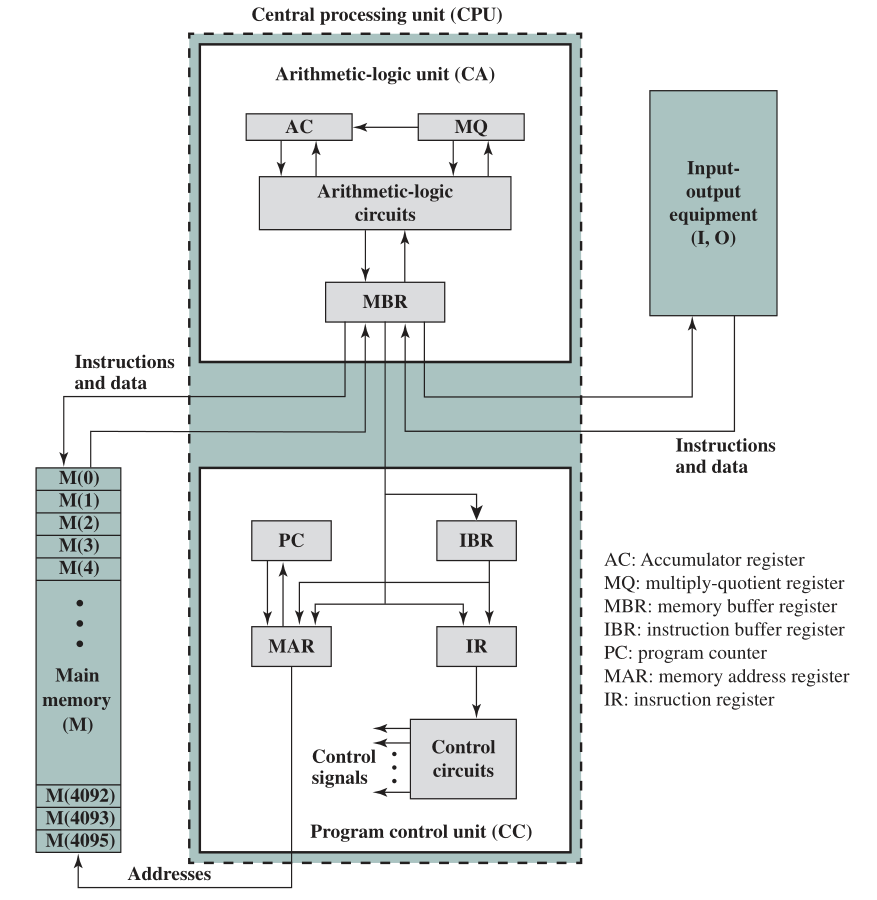
\includegraphics[width=0.58\textwidth]{ias.png}
\end{figure}

Para se explicar a estrutura do IAS, deve-se atentar a 5 partes principais:

\begin{enumerate}
    \item Um computador terá de ser capaz de executar as
	operações elementares básicas (adição, subtração, multiplicação,
	divisão). Normalmente, para essas funções são criadas unidades
	específicas para tais, comportadas em uma unidade maior
	centralizadora denominada CA ou unidade lógica e aritmética.

    \item Um computador terá de ser capaz de dar sequenciamento adequado as
	suas operações, instruções e as instruções de controle (comandos que
	regem o próprio sequenciamento do computador). Á essas undides é
	denomiada uma unidade central chamada CC ou controle central.

	As partes 1) e 2) juntas são chamadas de C. 

    \item Um computador terá a necessidade de processar sequências longas de
	operações, que, geralmente, não conseguem ser efetuadas em uma única
	leva de comandos. Logo, requer-se uma unidade que armazene dados por
	períodos duráveis para resolver problemas mais complexos, como
	cálculos.

	Essa unidade é denominada M ou memória.

	Analogamente ao funcionamento do corpo humano, essas três partes podem
	ser comparadas a parte cognitiva do corpo. Ou seja, a unidade lógica e
	aritmética, o controle central e a memória são o conjunto pensante do
	computador. Mas, assim como o corpo humano, se faz necessário a
	comunicação com o mundo externo, tal é feito por um canal denominado
	meio de gravação de sáida do dispositivo ou R, de modo que as últimas
	duas partes interagem com esse canal para satisfazer a necessidade de
	interação com o externo. 

    \item A parte de entrada do meio R, a qual deve transferir as informações
	desse para dentro de M e C é chamada de entrada ou I. É de boa prática a
	entrada passar os dados para dentro de M e nunca diretamenta para C. 

    \item Similarmente, a parte de saída do meio R, a qual deve transferir as
	informações de M e C para o meio R, é chamada de saída ou O. É de boa
	prática, também, a saída passar de M para R, assim, nunca diretamente
	por C. 
\end{enumerate}

Assim, resumidamente, temos a memória principal, que armazena dados e
instruções; a unidade lógica e aritmética (ALU), que opera os binários; a
unidade de controle, que interpreta e executa instruções e, por fim, o
equipmaneto de saída (E/S), que conecta o meio interno ao meio externo do
computador. \\

Como já antes dito, o modelo de IAS reflete em grande parte dos computadores atuais, por isso sua importância no mundo da computação.

\subsection{Endereçamento de memória}
O IAS possui 4.096 locais de armazenamento chamados de palavras, sendo esses dados ou instruções, cada um com 40 bits. As palavras são dividas em duas: palavra de número e palavra de instrução. \\

\begin{itemize}
	\item\quad 1) Palavra de número: contém um bit de sinal e outros 39 de armazenamento para o número. \\
	\item\quad 2) Palavra de instrução: pode conter duas instruções de 20 bits, cada uma contendo um opcode de 8 bits - referência que um processador possui para uma determinada instrução - e 12 bits de endereço de memória.
\end{itemize}

% Arrumar posição da imagem
%\begin{figure}[hb]
%   \caption{Figura 2: Tipos de palavras.}\textbf{}
%   \centering
%  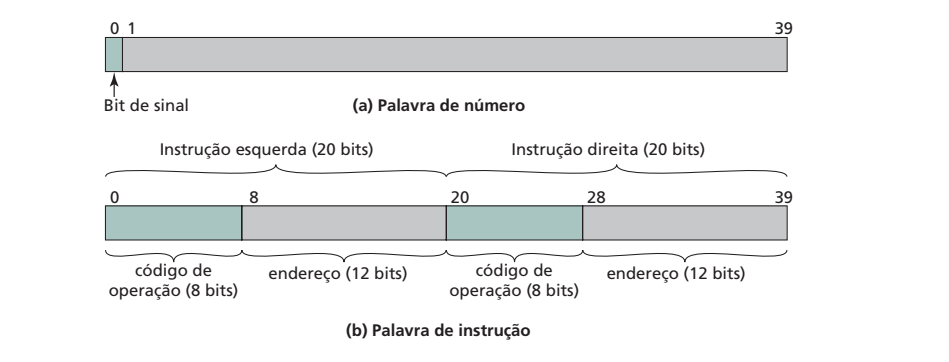
\includegraphics[width=0.75\textwidth]{palavras.png}
%\end{figure}

\subsubsection{Registradores}
Passando para as unidades menores do computador IAS, tem-se os locais de armazenamento da unidade de controle e da ALU, chamados de registradores.

\begin{itemize}
	\item Registrador de buffer de memória (MBR): é o local onde permanece a palavra a ser armazenada na memória ou enviada à unidade E/S, como também é o local para receber a palavra a partir da E/S ou a partir da memória.
	\item Registrador de endereço de memória (MAR): local que contém o endereço da memória da palavra a ser escrito ou lido pelo MBR.
	\item Registrador de instruções (IR): contém o opcode de 8 bits da instrução que está sendo executada.
	\item Registrador de buffer de instrução (IBR): mantém temporariamente a instrução da direita da palavra da memória.
	\item Contador do programa (PC): mantém o próximo par de instruções a ser buscado na memória.
	\item Acumulador (AC) e quociente-multiplicador (MQ): registradores usados para realizar as operações da ALU, sendo o AC o que mantém os bits mais significativos e o MQ os bits menos significativos.
\end{itemize}

\subsection{Ciclos do IAS}
\subsection{Segunda geração: Transístores}
\subsection{Terceira geração: Circuitos Integrados}
\subsection{Gerações posteriores}

\section{Aplicações} 
\subsection{Arquitetura x86} 
\subsection{Sistemas Embarcados}
\subsection{Arquitetura ARM} 
\subsection{Computação em Nuvem}

\end{document}
